%My header and style options
\documentclass[a4paper, twocolumn, titlepage]{article}
\usepackage[slovene]{babel}
\usepackage[utf8]{inputenc}
\usepackage[T1]{fontenc}

%\usepackage{vicent}
%\usepackage[0T1]{fontenc}

%custom colour package
\usepackage[usenames, dvipsnames]{xcolor}

%graphics, captions etc.
\usepackage[pdftex]{graphicx}
\usepackage{amssymb, float, amsmath, fullpage}

%to get the colourful hyperlinks ... not just square boxes around them ...
\usepackage{hyperref}
\hypersetup{
	colorlinks=true,
	linkcolor=black!60!red,
	citecolor=black!60!green,
	urlcolor=black!60!cyan,
	filecolor=black!60!magenta
}

%set up custom captions
\usepackage{caption}
\captionsetup{
	font=small,
	margin=10pt,
	labelfont=it,
%	labelsep=endash,
	format=hang,
	width=0.7\textwidth
}

%bibliography
%\usepackage[round]{natbib}

%LOOKS WAY BETTER WITHOUT THESE ... :P
%costum matter fonts and section fonts
%\usepackage{mathpazo}
%\usepackage{sectsty}
%\allsectionsfont{\LARGE\sffamily\bfseries}

\newcommand{\parc}[2]{
	\ensuremath{\frac{\partial#1}{\partial#2}}
}

\newcommand{\vac}[1][\phi]{
	\ensuremath{\langle#1\rangle}
}

%\renewcommand{\to}{
%	\ensuremath{\longrightarrow}
%}

% New definition of square root:
% it renames \sqrt as \oldsqrt
\let\oldsqrt\sqrt
% it defines the new \sqrt in terms of the old one
\def\sqrt{\mathpalette\DHLhksqrt}
\def\DHLhksqrt#1#2{%
\setbox0=\hbox{$#1\oldsqrt{#2\,}$}\dimen0=\ht0
\advance\dimen0-0.2\ht0
\setbox2=\hbox{\vrule height\ht0 depth -\dimen0}%
{\box0\lower0.4pt\box2}}

\newenvironment{myfig}[2][10cm]
{
	\vspace{-20pt}
	\begin{figure}[H]
		\begin{center}
			\includegraphics[keepaspectratio=1, width=#1]{#2}
		\end{center}
		\vspace{-24pt}
}
{
	\end{figure}
	\vspace{-6pt}
}

\renewenvironment{abstract}[1][1.0]
{
	\begin{center}
		{\bf Povzetek}\\[12pt]
		\begin{minipage}{#1\textwidth}
}
{
		\end{minipage}
	\end{center}
}

\newcommand{\rot}{
	\ensuremath{\vec{\nabla}\times}
}

\renewcommand{\div}{
	\ensuremath{\vec{\nabla}\cdot}
}

\newcommand{\ve}{
	\ensuremath{\vec{E}}
}

\newcommand{\vb}{
	\ensuremath{\vec{B}}
}

\newcommand{\w}{
	\ensuremath{\omega}
}

\renewcommand{\d}{
	\ensuremath{\mathrm{d}}
}

\begin{document}

%titlepage
\begin{titlepage}
	\begin{figure}[H]
		\centering
		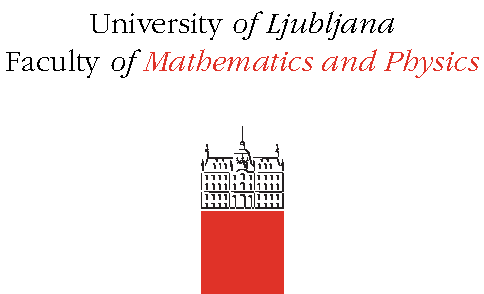
\includegraphics[width = 7cm, keepaspectratio=1]{pics/logo.pdf}\\[12pt]
		{\sc Oddelek za fiziko}\\[4cm]
	\end{figure}
	\begin{center}
		\large{Seminar -- 2. letnik 2. bolonjske stopnje}\\[0.5cm]
		\LARGE\textbf{Masivna elektrodinamika}\\[1.0cm]

		\vspace{0.0cm}

		\begin{minipage}{0.4\textwidth}\small
			\begin{flushleft}
				\textsc{Avtor:}\\[0.2cm]
				Jože Zobec
			\end{flushleft}
		\end{minipage}
		\begin{minipage}{0.4\textwidth}\small
			\begin{flushright}
				\textsc{Mentor:}\\[0.2cm]
				Prof. Dr. Borut Bajc
			\end{flushright}
		\end{minipage}
	\end{center}

	\vspace{4.5cm}

	\begin{abstract}
		Kot je verjetno potrebno venomer, so ob zori teorije o elektromagnetnem polju znanstveniki novosti
		sprejemali z zdravo mero dvoma. Tako so dlakocepili ob podrobnostih, ki so poznejše fizike privedle
		do možnosti neničelne mase fotona, katere eksperimentalno zaenkrat še ne moremo zanemariti. V tem
		seminarju bom na kratko opisal različne mehanizme, po katerih lahko foton dobi maso in naredil
		zgodovinski pregled meritev le-te.
	\end{abstract}
	
	\vfill

	\centering{\footnotesize Ljubljana, \today}
\end{titlepage}

%table of contents, obviously ...
%\tableofcontents

\pagebreak

\section{Uvod}

Newtonova teorija gravitacije je s svojo učinkovitostjo ter preprostostjo narave presunila mnoge tedanje mislece in
služila za navdih novincem, ki so se tedaj ravno pričeli ukvarjati z elektrodinamiko. Predpostavka je bila, da
električna sila med naboji prav tako pada z $r^{-2}$, tako kot gravitacijska. Nekateri so temu oporekali in so
poskušali z $r^{-2 + \alpha}$, malenkost, ki je povezana prav z maso fotona.~\cite{nieto2}

Fiziki francoske šole so se o tem nekako največ spraševali. Med njimi prednjači Proca, ki je prvi zapisal ekvivalent
Maxwellovih enačb za masivne fotone~\cite{nieto1,over}. Za njim so se s tem ukvarjali Stueckelberg~\cite{over,nieto1},
de Broglie~\cite{nieto1,over}, in med drugimi tudi Schroedinger~\cite{nieto1}.

S pojavom kvantne elektrodinamike so poskušali slednjo uporabiti za masivne fotone, pri čemer so naleteli na
različne nevšečnosti, pri čemer so pričeli z razvojem novih teoretičnih mehanizmov, s katermi bi foton dobil maso
in hkrati ohranil lepe lastnosti brezmasne elektrodinamike.

Masivna elektrodinamika je tudi dandanes zanimiva, ker s seboj prinaša vdaljnose\v zne posledice tudi v primeru, ko je masa
fotona zelo majhna~\cite{over}

\section{Začetki elektrodinamike}

Maxwellove enačbe so nas dosegle konec devetnajstega stoletja, nekaj desetletij za tem, jih je Proca prepisal v obliko,
ki zado\v s\v ca neni\v celni fotonski masi. Ena\v cbe se potem glasijo

\begin{align}
	&\div\ve = \rho/\varepsilon_0 - m^2\varphi, \qquad \div\vb = 0, \notag \\
	&\rot\ve = \parc{\vb}{t}, \qquad \rot\vb = \mu_0\vec{\jmath} + \frac{1}{c_0^2}\parc{\ve}{t} - m^2\vec{A},
	\label{eqn:max-proca}
\end{align}

kjer je $c_0 = 1/\sqrt{\varepsilon_0\mu_0}$ \v se vedno dobro definirana in nespremenjena. Kot vidimo, so ena\v cbe Proca
v Lorentzovo kovariantni obliki nespremenjene za dualni napetostni tenzor elektromagnetnega polja, medtem ko dobi samo
napetostni tenzor masne popravke, 

\begin{equation}
	\partial_\nu F^{\mu\nu} + m^2 A^\mu = \jmath^\mu.
	\label{eqn:proca}
\end{equation}

\v Ce ena\v cbo \eqref{eqn:proca} diferenciramo, lahko od ondod dobimo pogoj za Lorentzovo umeritev, $\partial_\mu
A^\mu$, ki nam reducira eno od \v stirih prostostnih stopenj $A^\mu$, od koder sledi, da gre za foton, s spinom $1$ in
maso $m$. Gostota Lagrangejeve funkcije\footnote{v nadaljevanju zaradi preprostosti raje kar Lagrange-ian}, $\mathcal{L}$,
se v tem primeru glasi

\begin{equation}
	\mathcal{L} = -\frac{1}{4}F_{\mu\nu}F^{\mu\nu} + \frac{1}{2}m^2A_\mu A^\mu.
	\label{eqn:proca-lagrangian}
\end{equation}

To polje lahko nato kvantiziramo, poka\v zemo, da zado\v s\v ca bozonski algebri.

Vendar kot vidimo \v ze v en. \eqref{eqn:max-proca} in \eqref{eqn:proca}, postanejo potenciali, torej $A_\mu =
(\varphi, \vec{A})$ fizikalne opazljivke v fiksni umeritveni skali (ki je v tem primeru Lorentzova). Taka teorija nima
umeritvene invariance.

\subsection{Posledice}

Kot sem namignil, ena\v cbe Proca s seboj prina\v sajo dolo\v cene nev\v se\v cnosti/inovacije:

\begin{itemize}
	\item{kr\v senje umeritvene invariance~\cite{nieto1,nieto2},}
	\item{svetlobna disperzija~\cite{nieto1,nieto2}}
	\item{kr\v senje (lokalne) ohranitve naboja~\cite{nieto2},}
	\item{dodatna longitudinalna komponenta elektromagnetnega sevanja~\cite{nieto1,nieto2},}
	\item{elektromagnetna interakcija ima kon\v cni doseg~\cite{nieto1,nieto2}}
\end{itemize}

kar nas lahko nekoliko preseneti -- da bo $\varphi$ dobil Yukawovo obliko gre pri\v cakovati, vendar kr\v senje ohranitve
naboja ni tako od muh. Pod kr\v sitvijo umeritvene invariance mislimo umeritveno invarianco prve vrste.

\subsubsection{Disperzijska relacija}

Svetlobna disperzija je najve\v cja razlika, ki jo je Proca povdarjal. Sam se ni menil, da bi ena\v cbe zapisal v
Lorentzovi kovariantni obliki in polja ni sku\v sal kvantizirati. Svetlobno disperzijo dobimo lahko na preprost na\v cin~\cite{nieto1}:

\begin{equation}
	k_\mu k^\mu = \frac{\w^2}{c_0^2} - k^2 = \mu^2 \propto p_\mu p^\mu = \frac{E^2}{c_0^2} - p^2 = m^2c_0^2,
	\label{eqn:disper}
\end{equation}

kjer je $\mu$ masa fotona, izra\v zena v enotah inverzne dol\v zine. V standarnih enotah velja $m = \mu\hbar/c_0$, vendar,
kot je tudi razvidno iz zgornjega izraza, pojma v enotah $\hbar = \varepsilon_0 = c_0 = 1$ sovpadata.

\v Ce sedaj ena\v cbo~\eqref{eqn:disper} diferenciramo, lahko poka\v zemo, da $\w \neq kc$, pri \v cemer je 
$c = c_g = \mathrm{d}\w/\mathrm{d}k \neq c_0$ ($c = c_g$ je grupna hitrost takega vala). Po prej\v snjih ena\v cb sledi

\[
	c = \frac{c_0}{\w}\sqrt{\w^2 - \mu^2c^2_0},
\]

od koder pa je o\v citno, da je $c = c (\w) \neq c_0$. Prve meritve, opravljene z namenom merjenja fotonske mase so bile
tako opravljene z merjenjem disperzijske konstante $\mu$. Odslej bomo vse pisali v prej omenjenih normiranih enotah, kjer
je $\hbar = c_0 = \varepsilon_0 = 1$.

\subsubsection{Kon\v cen doseg}

Ni mu bilo o\v citno, da bi bila elektrodinamika tako zaradi Yukawovega potenciala kon\v cna in da bi to nato prevedlo v
lokalno kr\v senje ogranitve elektri\v cnega naboja. Procovim naslednikom je po Yukawovi napovedi `mezona' postalo jasno,
da bi dobili prav to. Prvo Procovo ena\v cbo lahko zapi\v semo v obliko, kjer so samo potenciali in tako dobimo v
stati\v cnem primeru brez nabojev~\cite{nieto2}

\[
	\big(\Box + m^2\big)\varphi = 0, \quad \Longrightarrow \quad \varphi \propto \text{e}^{-\mu r}/r.
\]

Tak potencial je karakteristi\v cen za interakcije kon\v cnega dosega, kot je na primer \v sibka interakcija.

\subsubsection{Kr\v senje ohranitve naboja}

Gaussov zakon za ohranitev naboja dr\v zi v primeru, ko imamo potencial oblike $\varphi \propto 1/r$. Fotonska masa to
lepo lastnost seveda takoj pokvari, saj se \v stevilo silnic, ki prebadajo zaklju\v ceno ploskev ne ohranja, ampak se
spreminja. \v Ce je ta ploskev na primer krogla, lahko zapi\v semo pretok elektri\v cnega polja kot

\begin{multline*}
	\Phi_e = \oint_{\partial V} \ve \cdot \d \vec{S} = \int_V \big(\div \ve\big)\ r^2\d r\ \d\Omega =\\
		- \int_V \nabla^2\varphi r^2 \d r \propto \int_V \nabla^2 \left(\frac{\text{e}^{-\mu r}}{r}\right)r^2 \d
		r = f(r).
\end{multline*}

\v Ce v prej\v snji ena\v cbi uporabimo ena\v cbe Proca~\eqref{eqn:max-proca} lahko dobimo veliko huj\v so posledico, in
sicer, da je lokalna ohranitev naboja kr\v sena, kar pa pomeni, da sama kontinuitetna ena\v cba za elektri\v cni naboj ne
dr\v zi ve\v c. To je zelo grda lastnost, ki pa se prikrade notri ravno kot posledica kr\v sitve Gaussovega zakona.

\subsubsection{Longitudinalna polarizacija fotonov}

Ta je dokaj enostavna: z disperzijsko relacijo lahko pove\v zemo $\vec{k}$, $\mu$ in $c_g$, ter ugotovimo, da obstaja
re\v sitev tudi ko $\vec{k} = 0$, v tem primeru ima $\vec{k}$ tri komponente in vse od teh so dovoljene -- se pravi ima
spinske re\v sitve vrtilne koli\v cine (v enotah $\hbar$) $\pm 1$ in pa $0$, katere prej ni bilo. Ta o\v citno predstavlja
longitudinalno polarizacijo.

\section{Stueckelbergov mehanizem}

V dvajsetih letih prej\v snjega stoletja je Stueckelberg demonstriral kako lahko splo\v snemu kompleksnemu vektorskemu
polju, ki ima simetrijo U(1) dodamo maso, ne da bi pri tem zlomili umeritveno invarianco ter hkrati ohranili
renormalizabilnost teorije. Njegove ideje so ostale v ozadju, a so pozneje slu\v zile za navdih Higgsovemu mehanizmu.
Njegovo idejo so seveda uporabili tudi za realno vektorsko polje, $A_\mu$, se pravi foton.

Stueckelberg si je mislil, da je tisto kar je najpomembnej\v se v teoriji to, da je umeritveno invariantna. Pri tem imamo
lahko ve\v c razli\v cnih umeritev: umeritve skale, umeritve faze \ldots Njegova teorija ohranja oboje. Trik za foton
uporabimo takole: ker vemo, da mora imeti masivno vektorsko polje s spinom 1 prisotne natanko 3 prostostne
stopnje\footnote{spine, polarizacije}, se mu je zdelo primernj\v se pri\v ceti z $A_\mu$, kot pa z $F_{\mu\nu}$. Ta ima
4 prostostne stopnje. Proca se je ene stopnje znebil s pomo\v cjo Lorentzove umeritve, Stueckelberg pa je tu raje vpeljal
novo skalarno poljae $B$, ki je povezano z $A_\mu$. Tako imamo naenkrat 5 prostostnih stopenj. Izka\v ze se, da lahko na
tem mestu postuliramo relacijo

\[
	\big[\partial_\mu A^\mu + mB(x)\big]^{(-)}|\phi\rangle = 0,
\]

kjer je $|\phi\rangle$ katerokoli fizikalno stanje, operatorji pa imajo gornji index `$-$', ki ponazarja da gre le za
anihilacijske operatorje. S tem se znebimo ene od prostostnih stopenj, ko pa polje kvantiziramo opazimo, da imamo
umeritveno svobodo, ki nam skupaj zreducira \v stevilo prostostnih stopenj na 3. Dovoljena umeritev je te vrste:

\begin{align*}
	A_\mu (x) &\to A_\mu (x) + \partial_\mu \Lambda (x), \\
	B (x) &\to B (x) + m\Lambda(x).
\end{align*}

Iz brezmasnega do masivnega fotona torej pridemo s tem trikom:

\begin{equation}
	A_\mu (x) \to A_\mu (x) - \frac{1}{m}\partial_\mu B(x),
\end{equation}

Lagrange-ian se v tem primeru zapi\v se tako:

\begin{multline}
	\mathcal{L} = -\frac{1}{4}F_{\mu\nu}F^{\mu\nu} + \frac{1}{2}m^2\Big(A_\mu - \frac{1}{m}\partial_\mu B\Big)^2 -\\-
		\frac{1}{2\xi}\big(\partial_\mu A^\mu + \xi mB\big)^2,
\end{multline}

kjer $\xi \in \mathbb{R}$ in predstavlja umeritev skale. Razlika od Lagrange-iana za brezmasne fotone je v drugem
\v clenu in v dodatku v \v clenu za fiksiranje skale (\v clen z $B$-jem v tretjem \v clenu).

Poleg tega, da ohranimo svobodo umeritve ima Stueckelbergov trik \v se eno lepo lastnost: $F_{\mu\nu} F^{\mu\nu}$ je enak,
saj se prispevki skalarnega polja ravno izni\v cijo.

\section{Higgsov mehanizem}

Higgsov mehanizem prav tako doda novo skalarno polje, vendar je tam ideja druga\v cna: vse skupaj je mogo\v ce prek
spontanega zloma simetrije.

Higgsovega mehanizma ne gre me\v sati s Higgsovim delcem, katerega kandidata so v leto\v snjem poletju odkrili v CERN-u.
Foton sam pripada grupi U(1) in za maso ne potrebuje takega mehanizma, in lahko maso dobi neodvisno.

Prva taka razlika od elektro\v sibkega Higgsa je ta, da je elektromagnetni Higgs tu elektri\v cno nabit delec. Njegov
naboj je sorazmeren z maso fotona.

Zaradi sorodnosti s superprevodniki bi v tem primeru tudi pomenilo, da je masa fotonov lahko temperaturno odvisna in pri
neki kriti\v cni temperaturi postane enaka ni\v c (superprevodna faza fotonov).

\section{Meritve}

Da bi izmerili ni\v celno maso fotona je ideal, katerega ne moremo nikdar dose\v ci, vendar kljub temu \v se vedno
potrebujemo neke vrste kriterij, ki nam pove, ali je izmerjena vrednost zadosti majhna, da lahko teorijo ovr\v zemo.
Zato se i\v s\v ce samo zgornjo mejo za maso, spodnjo namre\v c lahko dobimo s Heisenbergovim principom
neenakosti~\cite{over}:

\begin{equation}
	\delta t \cdot \frac{\delta E}{\hbar} = \delta t \cdot \frac{mc_0^2}{\hbar} = \delta t \cdot \mu c_0 \sim 1,
\end{equation}

kjer za $\delta t$ vstavimo starost vesolja ($10^{17}$ sekund) in dobimo spodnjo mejo za maso fotona \hbox{$m \sim
10^{-69}$ kg}.
\v Ce je masa fotona manj\v sa od tega, pomeni da jo lahko pripi\v semo kvantnim fluktuacijam, katere pa \v ze namo
pojasniti in bi bile meritve odve\v c.

Meritve lahko združimo nekako v tri razrede:
\begin{itemize}
	\item{Laboratorijske -- opravljene so v skrbno nadzorovanem okolju na Zemlji.}
	\item{Meritve znotraj na\v sega oson\v cja -- opravljene so s pomočjo satelitov.}
	\item{Kozmološke -- s teleskopi opazujemo razna nebesna telesa, ki so zelo oddaljena.}
\end{itemize}

Laboratorijske lahko nato razdelimo še na `kvantne' in `klasične', kjer pod klasične mislimo spremembe glede na Maxwellovo
elektrodinamiko.

\subsection{Laboratorijske meritve}

Vse skupaj se je pričelo s preverjanjem odvisnosti $F \propto r^{-2}$. Ker so fiziki tedaj pluli v neznane vode, so dopuščali
popravek temu, tj. $r^{-2 + \alpha}$. V primeru fotonske mase se izkaže, da je $\alpha = \alpha (r)$, ker je potencial masivnega
fotona oblike $\varphi \sim \text{e}^{-\mu r}/r$. Odklone od zakona $r^{-2}$ so merili predvsem na dva načina: \textbf{(a)} direktno
z meritvijo pojemanja sile z razdaljo (Coulomb, Robinson), \textbf{(b)} z merjenjem odsotnosti sil zunanjih lupin znotraj
sferičnega objekta\footnote{Kot je Newton demonstriral za svojo teorijo gravitacije, ima sila obliko $F \sim r^{-2}$, kar prinaša s
seboj lepe lastnosti: če smo namreč na neki globini $h$ pod Zemljo, na nas deluje le sila Zemlje z radijem $R - h$, se pravi, da
nam zunenje lupine z debelino $h$ ni treba upoštevati, ker je njen prispevek natanko 0. Ko so to prevedli na meritve električnih
sil, v veliko nabito kroglo zaprli manjšo in opazovali interakcije med njima -- po navadi pretečen električni naboj.} in
merjenjem oblike električnega potenciala (Cavendish, Maxwell \ldots). Te meritve so očitno laboratorijske. V zadnjih dveh, treh
desetletjih so pričeli meriti tudi kvantne posledice.

\subsubsection{Klasične meritve}

Meritve odklona tipa $F \sim r^{-2 - \alpha}$ lahko povežemo z meritvami fotonske mase, ker lahko izpeljemo enakost~\cite{over}

\begin{equation}
	\frac{\varphi(r) - \varphi(a)}{\varphi(a)} \approx \alpha \approx -\frac{1}{6}\mu^2(a^2 - r^2),
\end{equation}

od koder lahko s poznavanjem dimenzij problema dobimo podatek o masi takega fotona.

Franklin (1755) je naredil prvi eksperiment, kjer je na nitki obsil majhno plutovinasto kroglico in dal, da je visela v nabit
kovinski lonček~\cite{over}. Ker ni bilo interakcije med njima, je Priestley (1767) sklepal, da sila pada s kvadratom razdalje,
tako kot Newtonova gravitacijska sila, ker bi se v tem primeru prispevki sil izničili. Eksperiment je bil zgolj kvalitativen in je
služil zgolj kot motivacija naslednikom.

Prvo kvantitativno obravnavo je naredil angleški fiziolog Robison (1769). Meril je odbojno silo med dvemi nabitimi palicami, ki jo
je uravnovesil z njuno privlačno gravitacijsko silo -- maso palic je namreč poznal. Izmeril je odklon $\alpha = 0,06$ in tudi
ugibal, da bi morala biti ta številka negativna za privlačno električno silo, zaradi česar je sklepal da je $r^{-2}$ res pravi
zakon. Rezultate je objavil šele leta 1801, 13 let za Coulombom, dasiravno je meritev opravil pred njim.

Coulombov poskus (1788) je bil bolj sofisticiran, meril je odbojno, kot tudi privlačno silo električno nabitih krogel s pomočjo
torzijske tehtnice. Odmik zaradi sile, je torej prenesel na odmik kota, ki ga je meril z zracalom, na katerega je imel usmerjen
svetlobni snop. Njegov rezultat je ustrezal $\alpha \leq 0,01$.

Vsi drugi poskusi klasični laboratorijski poskusi so bili sorodnega tipa, kot si ga je zamislil Cavendish. Njegov eksperiment je
bil zastavljen takole: imel je dve koncentrični krogli, zunanja je bila sestavljena iz dveh polobel, da se jo je lahko razprlo.
Znotraj sta bili povezani z elektrostatsko napravo~\cite{over}. Povezavo so nato nanadoma prekinili, zunanjo kroglo previdno odprli
in preverili, če je naboj notranje krogle res enak 0. Cavendish je dobil rezultat $\alpha \leq 0,02$, torej slabše od Coulomba.

Isti poskus pozneje opravil tudi Maxwell in za rezultat dobil $\alpha \approx 5 \times 10^{-5}$.

Poskus so opravili nato z razimi koncentričnimi telesi, ne le s kroglami, saj v primeru $r^{-2}$ Gaussov zakon velja za vse oblike.
Tako so isto stvar ponovili s kockami, ikozaedri in na izmeničnih napetostih s fazno vpeto zanko (tu napiši kdo so bili tile
ljudje, kdaj so bili tile poskusi opravljeni itd.).

V laboratorijih so skušali opraviti tudi poskuse svetlobne disperzije, vendar se bolj obnesejo pri velikih razdaljah in zategadelj spadajo
med astronomska opazovanja.

\subsubsection{Kvantni poskusi}

To so poskusi, katere je fizikom šele pred kratkim uspelo narediti in so privlačni zaradi tega, ker jih lahko izvajamo v nadzorovanem okolju.

Meritve, ki so bile opravljene z zadovoljivo natančnostjo, so bile Aharonov-Bohm efekt in defekti giromagnetnega razmerja elektrona.
Pri giromagnetnem razmerju je stvar nekam zgoljufana. Masa fotona, dobljena na ta način, je namreč zelo groba ocena in ne namenska meritev
fotonske mase. Ocenijo jo namreč tako, da vse odstopanje meritve od teoretične vrednosti, ki jo napoveduje kvantna elektrodinamika za
brezmasni foton, pripišejo fotonski masi. Vrednost, ki so jo dobili na ta način je $m \approx 10^{-54}$ g~\cite{over}.

Pri Aharonov-Bohm efektu gre za pravo in bolj sofisticirano meritev. Zaradi efektov kvantne mehanike se je izkazalo, da lahko namreč merimo
vpliv vektorskega potenciala magnetnega polja na fazo interferenčne dveh vzporednih elektronskih curkov. Ta efekt ima teoretično napoved za
neničelno, kot tudi ničelno maso fotona. Poskus izgleda takole: \emph{povej kako izgleda poskus in dodaj še sliko. Prav tako napiši, kolikšna
je eksperimentalna vrednost. Povej kdo vse je to meril.} Najnatančnejši rezultat so dobili Williams, Faller in Hill (1965),
$m \lesssim 10^{-14}$ eV $\equiv 2\times 10^{-47}$ g~\cite{nieto2}.

Take meritve postajajo končno primerljive z opazovanji iz vesolja in
bodo morda prinesle merjenje fotonske mase nazaj na zemljo.

Kot zanimivost naj dodam tudi to, da so po navdihu Higgsovega mehanizma za foton naredili tako imenivani "`kriogenski"' poskus tipa Cavendish.
Teoretični princip za temperaturno odvisnost sta napisala Primack in Scher~\cite{nieto2},
opravili pa so ga Ryan, Acceta in Austin (1985) in dosegeli $m \leq (1,5 \pm 1,38) \times 10^{-42}$ g, pri temperaturi
$1,36$ K~\cite{over}.

\subsection{Meritve v našem osončju}

Fiziki prejšnjega stoletja so videli, da je Maxwellova elektrodinamika zelo natančna v skoraj vseh pogledih. Možnosti za nadgradnjo so videli
bodisi pri zelo velikih razdaljah\footnote{zelo dolga valovna dolžina} ali pa rešitve po dolgem času.

Schroedinger (1943)~\cite{nieto1} se je zato odločil, da bo meril obliko silnic zemeljskega magnetnega polja. Dipolni moment zemlje bi po
Maxwellu imel obliko $1/r^3$, vendar pa mora zaradi Yukowovega potenciala padati hitreje. Defekt bi bil najbolje viden na ekvatorju.
Schroedinger je uporabil že obstoječe meritve iz leta 1922, ki jih je objavil gospod Schimidt leta 1924. Leta 1955 sta se z Bassom odločila,
da bosta rezultat pomnožila s faktorjem $2$ in dobila mejo $m \leq 10^{-47}$ g~\cite{nieto1}.

Schroedingerjevo meritev sta ponovila A.S. Goldhaber in M.M. Nieto (1968) in dobila oceno $m = 4 \times 10^{-48}$ g~\cite{nieto1, over}.

Iste poskuse so pozneje opravili za večja telesa, kot je tudi Schroedinger predlagal. Najboljši rezultat bi po njegovem mnenju dal Jupiter,
saj je nejvečji med planeti. To je storil Davis (1975) s svojo ekipo, uporabili so rezultate sonde Pioneer in dobili rezultat
$m \lesssim 4\times10^{-16}$ eV $\equiv 7 \times 10^{-49}$ g~\cite{nieto2,over}.

S pomočjo disperzije optične svetlobe je de Broglie napovedoval mejo $m \leq 10^{-39}$ kg~\cite{nieto2}. Pozneje so jo izmeril Kroll,
ki pravi $m \lesssim 3 \times 10^{-13}$ eV $\equiv 4 \times 10^{-46}$ kg~\cite{nieto2}.

Opraviljene so bile še druge meritve, ki so predolge za ta seminar, kot na primer vplivi mase na sončev veter (Ryutov 2007,
$m \lesssim 10^{-18}$ eV $\equiv 20\times10^{-51}$ g).

\subsection{Kozmološke meritve}

Pod tem imenom je mišljeno na meritve, ki so galaktičnih razsežnosti, izven našega osončja. Meri se predvsem magnetno polje in
vektorski potencial
iz galaktičnega jedra~\cite{over}, obliko svetlobnega snopa iz pulzarjev~\cite{nieto1} in oblike meglic~\cite{nieto2}.

Najzanimivejša metoda je metoda, ki jo je predlagal
Lakes (1998) za merjenje magnetnega vektorskega potenciala. Magnetno polje je daleč od galktičnega jedra
skoraj konstantno, prav tako tudi vektorski potencial, ki je zaradi mase fotona opazljivka v Lagrange-ianu. Zaradi vrtenja Zemlje okrog
svoje osi s frekvenco $\w$ in neničelnega ambientalnega vektorksega potenciala, bi na zemljo deloval navor

\[
	\vec{M} \propto \vec{\w} \times m^2\vec{A}
\]

Smer $\vec{A}$ lahko sklepamo iz smeri vrtenja naše galaksije, dolžino pa je ocenil s z $|\vec{A}| \approx L|\vec{B}|$, kjer je $L$ oddaljenost
od galaksije. Ravno zaradi teh predpostavk ne moremo biti gotovi v rezultate meritve -- lahko da je $\vec{A}$ veliko manjši od $LB$, prav
tako ne vemo če je magnetno polje res homogeno. Kljub temu so po njegovem predlogu naredili meritev in dobili
$m \lesssim 7 \times 10^{-20}$ eV $\equiv 10^{-52}$ g~\cite{nieto2}. Ker seveda ne poznamo prave vrednosti $\vec{A}$ je to zelo groba ocena.
Če je $|\vec{A}|$ zelo majhna vrednost, ne bi opazili mase fotona, tudi če bi bila zelo velika. Prav tako ne moremo reči, da je celoten
prispevek $\vec{A}$ posledica vektorskega potenciala galaksije.

Higgsov mehanizem bi bil tudi tukaj -- v režimu, ki bi bil analogen superprevodniku tipa II, bi imel foton maso lahko v zelo viskih energijah,
temperaturah, torej v zgodnjem vesolju~\cite{nieto2}.

\begin{thebibliography}{9}
	\bibitem{nieto2}
	A. S. Goldhaber and M. M. Nieto,
	"`Photon and Graviton Mass Limits"',
	arXiv:0809.1003v5 [hep-ph],
	(2010)

	\bibitem{nieto1}
	A. S. Goldhaber and M. M. Nieto,
	"`Terrestrial and Extraterrestrial Limits on The Photon Mass"',
	Rev. Mod. Phys. {\bf 43}, 277-296,
	(1971)

	\bibitem{stueckelberg}
	H. Ruegg and M. Ruiz-Altaba,
	"`The Stueckelberg Field"'
	arXiv:hep-th/0304245v2,
	(2003)

	\bibitem{higgs}
	E. Adelberger, G. Dvali and A. Gruzinov,
	"`Photon Mass Bound Destroyed by Vortices"',
	arXiv:hep-ph/0306245v2,
	(2003)

	\bibitem{over}
	G. Spavieri, J. Quintero, G.T. Gillies and M. Rodriguez,
	"`A survey of existing and proposed classical and quantum approaches to the photon mass"',
	Eur. Phys. J. D {\bf 61} 531-550,
	(2011)
\end{thebibliography}

\end{document}

